%\RequirePackage{snapshot}
\documentclass[a4paper,KOMA,landscape]{powersem}
\usepackage[display,stmo]{ifmslide}
\usepackage{soul}
%\usepackage[dvips]{graphicx}
%% user definitions
\newcommand{\ifmslide}{{\code{ifmslide.sty}}}
\newcommand{\tp}{{\code{texpower{}} \cite{texpower} }}
\newcommand{\hf}{{\code{hyperref{}} \cite{hyperref} }}
\hypersetup{pdfauthor={Henrik Frisk and Stefan �stersj�}}
\hypersetup{pdftitle={Negotiating the Musical Work. \\An empirical study on the
inter-relation between composition, interpretation and performance.}}
\hypersetup{pdfsubject={presentation}}
\hypersetup{bookmarksopen={false}}
\hypersetup{pdfpagemode={None}}

\IfFileExists{cmtt.sty}{\usepackage[override]{cmtt}%
                        \newcommand{\bs}{{\mtt\\}}}{%
                        \newcommand{\bs}{{$\setminus$}}}%

\panelposition{bottom}
\panellogo{Ulomacvnege}
\releaselogo
\freelogo(190,135)[5cm]

%%%%%%%%%%%%%%%%%%%%%%%%%%%%%%%%%%%%%%%%%%%%%%%%%%%%%%%%%%%%%%%%%%%%
%\usepackage{thumbpdf}
%%%%%%%%%%%%%%%%%%%%%%%%%%%%%%%%%%%%%%%%%%%%%%%%%%%%%%%%%%%%%%%%%%%%
\begin{document}
\headskip=12mm
\sffamily

\orgname{Malm\"{o} Academy of Music - Lund University}

\title{\begin{minipage}[t]{0.98\textwidth}\begin{center}
      {\mdseries Negotiating the musical work I. \\
					   Studies in interaction and
					   communication - theory and method.\\}
\vspace{1cm}
     {\mdseries EMS 2006, Beijing}
    \end{center}\end{minipage}}

\author{\scalebox{1}[1.3]{Henrik Frisk \& Stefan \"{O}stersj\"{o}}}

\address{\href{mailto:henrik.frisk@mhm.lu.se}
  {henrik.frisk@mhm.lu.se} \href{mailto:stefan\_ostersjo@hotmail.com}{stefan\_ostersjo@hotmail.com}}
%\orgurl{http://www.henrikfrisk.com}
\slidepagestyle{panel}
%%%%%%%%%%%%%%%%%%%%%%%%%%%%%%%%%%%%%%%%%%%%%%%%%%%%%%%%%%%%%%%%%%%%
\begin{slide}
 \maketitle
\end{slide}
%%%%%%%%%%%%%%%%%%%%%%%%%%%%%%%%%%%%%%%%%%%%%%%%%%%%%%%%%%%%%%%%%%%%
\centerslidesfalse
\begin{slide}
  \section{Overview}
  \pause
  \liststepwise
      {
        \begin{itemize}
	 \item{Developing hybrid methods for artistic research.}
	 \step{\item{The ontology of the musical work.}}
	 \step{\item{Discussion of computer-performer interaction.}}
	 \step{\item{Summary}}
	\end{itemize}
      }
\end{slide}
%%%%%%%%%%%%%%%%%%%%%%%%%%%%%%%%%%%%%%%%%%%%%%%%%%%%%%%%%%%%%%%%%%%%

%%%%%%%%%%%%%%%%%%%%%%%%%%%%%%%%%%%%%%%%%%%%%%%%%%%%%%%%%%%%%%%%%%%%
\begin{slide}
  \section{Introduction}
  \subsection*{Purpose of the study.}
  \pause
  \liststepwise
      {
        \begin{itemize}
	 \item{The musical work before its ultimate notation and performance.}
	 \step{\item{Mixed media music.}}
	 \step{\item{Wish to gain a deeper understanding of the
	      underlying processes in the communication between the
	      composer and the performer.}}
	 \step{\item{Making use of this knowledge when constructing
	      interactive performance systems.}}
        \end{itemize}
      }
\end{slide}
%%%%%%%%%%%%%%%%%%%%%%%%%%%%%%%%%%%%%%%%%%%%%%%%%%%%%%%%%%%%%%%%%%%%

%%%%%%%%%%%%%%%%%%%%%%%%%%%%%%%%%%%%%%%%%%%%%%%%%%%%%%%%%%%%%%%%%%%%
\begin{slide}
  \section{The ontology of the musical work}
  \liststepwise {
  \step { 
  \begin{itemize}
   \item {Trevor Wishart: A split of the musician into two agents. \cite{wis96}}
   \step{\item {Nelson Goodman: Autographic vs. Allographic. \cite{goodman68}}}
   \step{\item {Paul Ric{\oe}ur: The world of the text.\\}}
	 \step{and... Interpretation during the act of writing.\cite{ric91}}
   \step{\item {Horacio Vaggione:\\
	 {\itshape So thesis and constraints are revealed through
	 perception. They are to be heard, first of all, by the composer
	 who is also a listener.} \cite{vaggione01}}}
   \step{\item {Performance interpretation: Construction vs. reproduction}}
   \step{\item {Peter Kivy: Different authenticities \cite{kivy}}}
   \step{\item {The technology of notation and computer programming.}}
  \end{itemize}
  }
  }
\end{slide}
%%%%%%%%%%%%%%%%%%%%%%%%%%%%%%%%%%%%%%%%%%%%%%%%%%%%%%%%%%%%%%%%%%%%

%%%%%%%%%%%%%%%%%%%%%%%%%%%%%%%%%%%%%%%%%%%%%%%%%%%%%%%%%%%%%%%%%%%%
\begin{slide}
 \section{Construction - Reproduction\\/ Composer - Performer}
      \liststepwise
      {

      \step
            {
	    Traditional view\\

              \begin{minipage}[h]{\textwidth}\begin{center}
                  {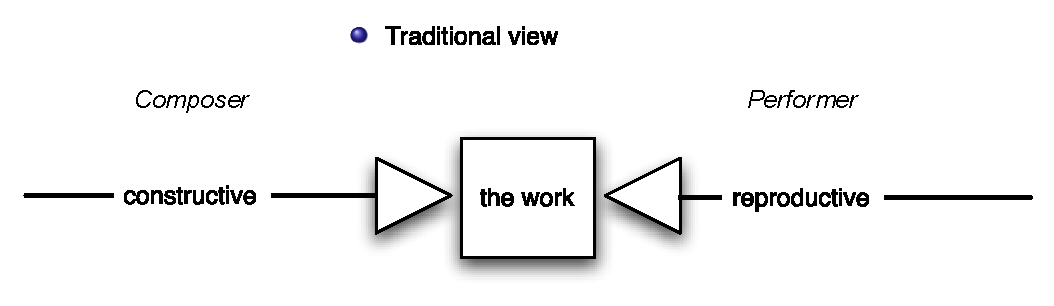
\includegraphics[width=0.9\textwidth]{img/cons-rep.pdf}} \end{center}
              \end{minipage}
            }
      }
\end{slide}
%%%%%%%%%%%%%%%%%%%%%%%%%%%%%%%%%%%%%%%%%%%%%%%%%%%%%%%%%%%%%%%%%%%%

%%%%%%%%%%%%%%%%%%%%%%%%%%%%%%%%%%%%%%%%%%%%%%%%%%%%%%%%%%%%%%%%%%%%
\begin{slide}
 \section*{Construction - Reproduction\\/ Composer - Performer}
	    Paul Ric{\oe}ur \cite{ric91}

              \begin{minipage}[h]{\textwidth}\begin{center}
                  {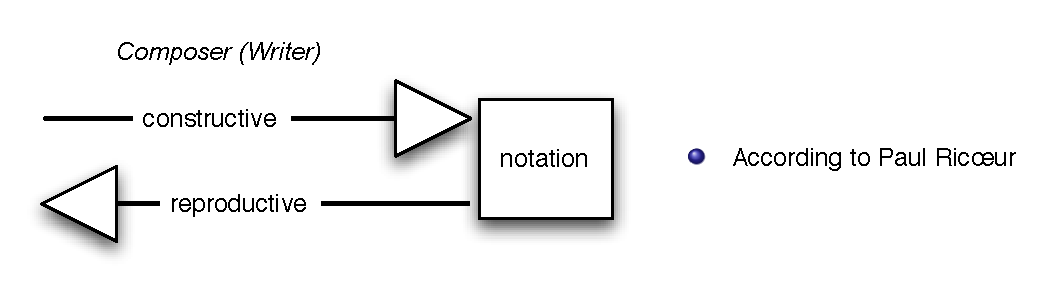
\includegraphics[width=0.5\textwidth]{img/cons-rep-ricoeur.pdf}} \end{center}
              \end{minipage}
\end{slide}
%%%%%%%%%%%%%%%%%%%%%%%%%%%%%%%%%%%%%%%%%%%%%%%%%%%%%%%%%%%%%%%%%%%%

%%%%%%%%%%%%%%%%%%%%%%%%%%%%%%%%%%%%%%%%%%%%%%%%%%%%%%%%%%%%%%%%%%%%
\begin{slide}
 \section*{Construction - Reproduction\\/ Composer - Performer}
	    Our experience of a more non-static inter-relation.

                            \begin{minipage}[h]{\textwidth}\begin{center}
							   {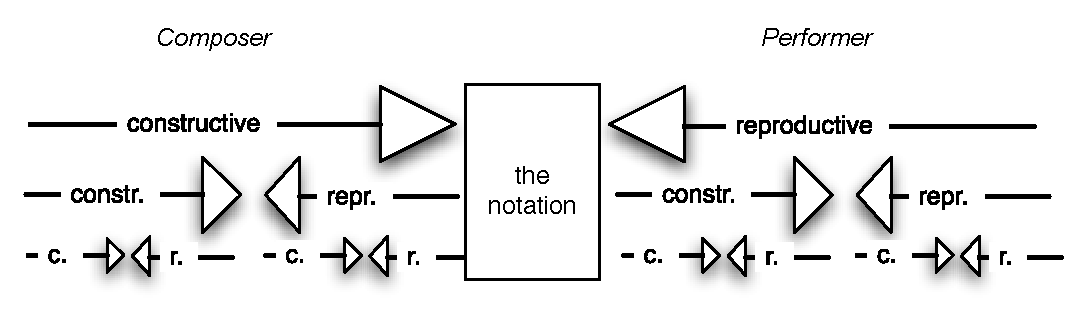
\includegraphics[width=0.9\textwidth]{img/cons-rep-rep-cons.pdf}} \end{center}
			    \end{minipage}
			    
\end{slide}
%%%%%%%%%%%%%%%%%%%%%%%%%%%%%%%%%%%%%%%%%%%%%%%%%%%%%%%%%%%%%%%%%%%%

%%%%%%%%%%%%%%%%%%%%%%%%%%%%%%%%%%%%%%%%%%%%%%%%%%%%%%%%%%%%%%%%%%%%
\begin{slide}
 \section{Methodology - hybrid methods.}
  \liststepwise {
\begin{itemize}
 \item{ Musical semiology.\\
      Drawing on Nattiez and Molino and their idea of tripartition - \\
      \emph{poietic} - \emph{neutral} - \emph{esthesic}}

  \step {\item{Qualitative research. Theorethical sampling
      vs. hermeneutics.\\
      Gadamer's notion of {\itshape Vorverstehen}; any kind of
      interpretation (of texts) involves an anticipated understanding of the
      analyzed object. \cite{gad60}\\
      Using a qualitative method when approaching the complex area of
      machine-musician interaction.}}

  \step{ \item{ Verbatim transcription of the video.\\
      Doing a verbatim transcription of video documentation from which a graph
      was extracted.}}

\end{itemize}  
   }
\end{slide}
%%%%%%%%%%%%%%%%%%%%%%%%%%%%%%%%%%%%%%%%%%%%%%%%%%%%%%%%%%%%%%%%%%%%

%%%%%%%%%%%%%%%%%%%%%%%%%%%%%%%%%%%%%%%%%%%%%%%%%%%%%%%%%%%%%%%%%%%%
\begin{slide}
  \section{Semiological approach.}
  \liststepwise { 
%
%  \step{\subsection*{Musical semiology}
%  \begin{itemize}
%   \item {Analytical understanding of the musical work in its entirety.}
%  \end{itemize}
%  }

  \step{\subsection*{Background to musical semiology}}
  \step{{\small The notion of a {\itshape 'single, well-defined item of information
      to be transmitted, all the rest being simply noise'} is
      {\itshape 'dangerously inaccurate and misleading as soon as we move from the
      artificial communication of information to a concrete act of human
      communication as a total social fact.'}} \cite{molino}}  
      
      \step{{\small  Duchamp: {\itshape two poles, the artist and the viewer. The intention of
      the artist holds no significance to the viewer.}}}

      \step{{\small Val\'{e}ry: {\itshape 'there is no guarantee of a direct
      correspondance between the effect produced by a work of art and the
      intentions of its creator'.}}} 
}
\end{slide}
%%%%%%%%%%%%%%%%%%%%%%%%%%%%%%%%%%%%%%%%%%%%%%%%%%%%%%%%%%%%%%%%%%%%

%%%%%%%%%%%%%%%%%%%%%%%%%%%%%%%%%%%%%%%%%%%%%%%%%%%%%%%%%%%%%%%%%%%%
\begin{slide}
  \section{Musical semiology}
  \liststepwise { 
  What is the nature of musical signification?
  \step{
  \begin{itemize}
   \item{''Music is a language that signifies itself.'' \cite{nat89}}
%	(referring
%	to N. Ruwet)}
   \step{\item{''Music - the unconsummated symbol.'' \cite{molino}}}
   \step{\item{''The signs are of interest to semiotics as social powers.'' -
   ``the cultural convention'' \cite{eco71}}}
   \step{\item{A subculture created by composer/peformer interaction?}}
  \end{itemize}
  }
  }
\end{slide}
%%%%%%%%%%%%%%%%%%%%%%%%%%%%%%%%%%%%%%%%%%%%%%%%%%%%%%%%%%%%%%%%%%%%

%%%%%%%%%%%%%%%%%%%%%%%%%%%%%%%%%%%%%%%%%%%%%%%%%%%%%%%%%%%%%%%%%%%%
\begin{slide}
  \section{The three dimensions}
  \liststepwise { 

  \step{...recognizing, elaborating, and articulating the three relatively
autonomous levels (poietic, neutral and esthesic) facilitates
knowledge of all processes unleashed by the musical work, from the
moment of the work's conception, passing through its 'writing down',
to its performance. \cite{nattiez}}  

       \step{A model of analysis on three levels:}
          \step
              {
                \begin{itemize}
		 \item{the poietic - the constructive phase}
                  \step{\item{the esthesic - the interpretative phase}}
                  \step{\item{the neutral - the trace}}
                \end{itemize}
              }
}
\end{slide}
%%%%%%%%%%%%%%%%%%%%%%%%%%%%%%%%%%%%%%%%%%%%%%%%%%%%%%%%%%%%%%%%%%%%

%%%%%%%%%%%%%%%%%%%%%%%%%%%%%%%%%%%%%%%%%%%%%%%%%%%%%%%%%%%%%%%%%%%%
\begin{slide}
  \section{The graph the communication.}
              \begin{minipage}[h]{\textwidth}
	       \begin{center}
	       {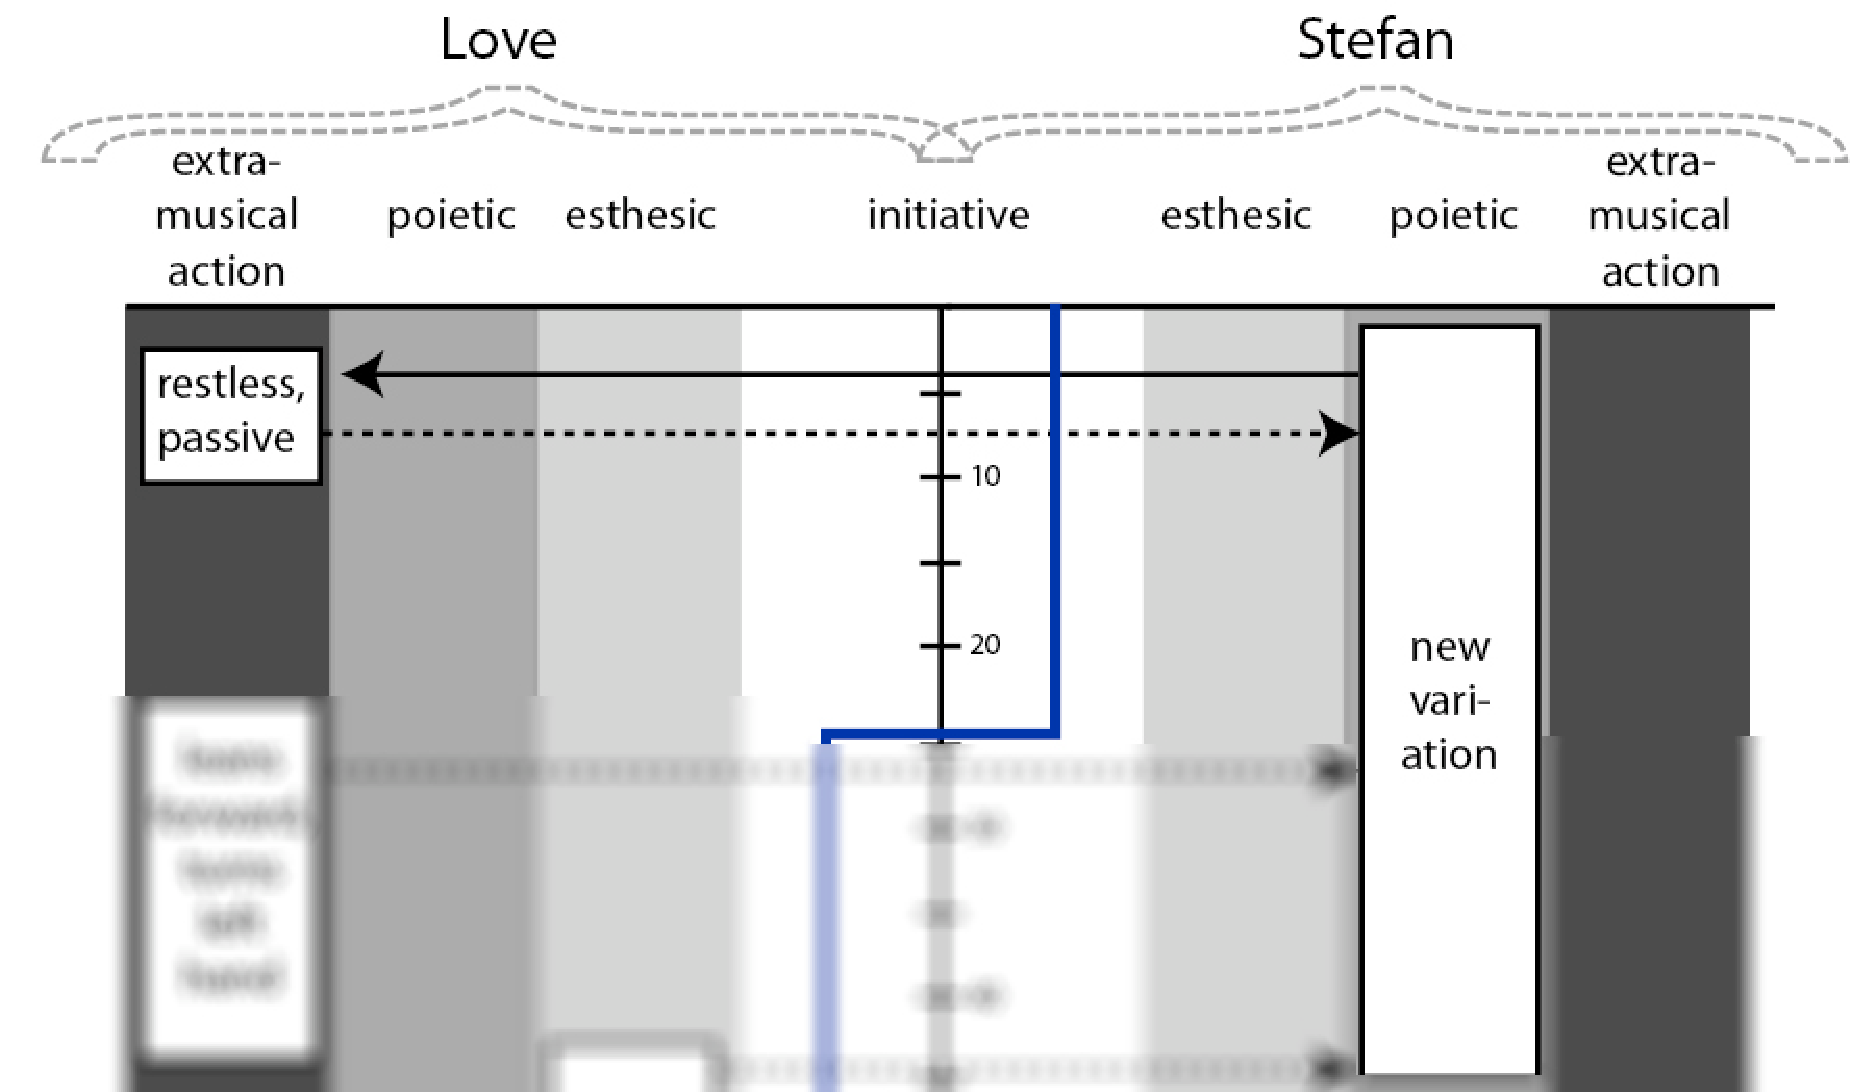
\includegraphics[width=0.75\textwidth]{img/timeline-section1.pdf}} 
	       \end{center}
              \end{minipage}
\end{slide}
%%%%%%%%%%%%%%%%%%%%%%%%%%%%%%%%%%%%%%%%%%%%%%%%%%%%%%%%%%%%%%%%%%%%

%%%%%%%%%%%%%%%%%%%%%%%%%%%%%%%%%%%%%%%%%%%%%%%%%%%%%%%%%%%%%%%%%%%%
\begin{slide}
 \section{The graph the communication.}
      \liststepwise
      {
      \step
            {
              \begin{minipage}[h]{\textwidth}
	       \begin{center}
		{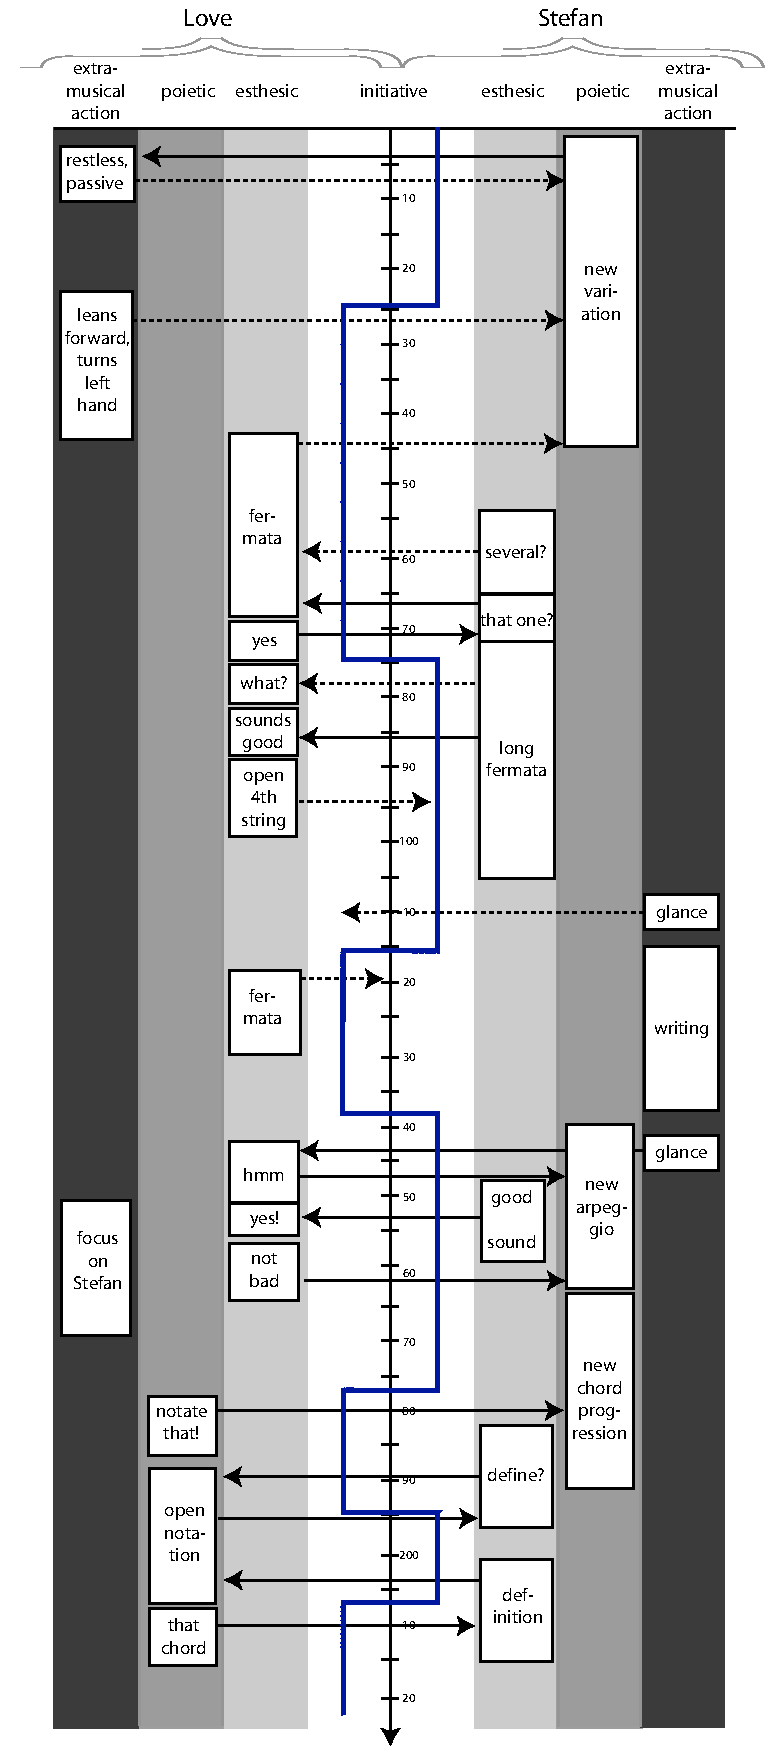
\includegraphics[width=0.2\textwidth]{img/timeline_horiz.pdf}}
	       \end{center}
              \end{minipage}
              }
      	      }
\end{slide}
%%%%%%%%%%%%%%%%%%%%%%%%%%%%%%%%%%%%%%%%%%%%%%%%%%%%%%%%%%%%%%%%%%%%

%%%%%%%%%%%%%%%%%%%%%%%%%%%%%%%%%%%%%%%%%%%%%%%%%%%%%%%%%%%%%%%%%%%%
\begin{slide}
  \section{Whose work? Whose performance?}
  \liststepwise {

  \step{Swapping of the roles?}

  \step{Roles of composer and performer overlap.}

      \step
            {
	    Conclusions from the analysis of the video:
	     \begin{itemize}
	      \item {Composition may be regarded as made up of a complex interaction between
		    esthesic and poietic processes.}
	      \step{\item {Performers similarly oscillate between these two modes of artistic
		    activity.}}
	     \end{itemize}
            }
	    }
\end{slide}
%%%%%%%%%%%%%%%%%%%%%%%%%%%%%%%%%%%%%%%%%%%%%%%%%%%%%%%%%%%%%%%%%%%%

%%%%%%%%%%%%%%%%%%%%%%%%%%%%%%%%%%%%%%%%%%%%%%%%%%%%%%%%%%%%%%%%%%%%
\begin{slide}
 \section*{Computer-Musician interaction.}
  \subsection{Reflections on the results of the empirical study.}
      \liststepwise
      {
      \step
            {
	     \begin{itemize}
	      \item {Noise in communication is not a problem.}
	      \step{\item {Direction is more important than
		    synchronicity.}}
	      \step{\item {The initiative can shift independently of the
		    esthesic and poietic processes.}}
	     \end{itemize}
            }
     	      }
\end{slide}
%%%%%%%%%%%%%%%%%%%%%%%%%%%%%%%%%%%%%%%%%%%%%%%%%%%%%%%%%%%%%%%%%%%%

%%%%%%%%%%%%%%%%%%%%%%%%%%%%%%%%%%%%%%%%%%%%%%%%%%%%%%%%%%%%%%%%%%%%
\begin{slide}
  \section{Current and future work.}
  \liststepwise { 

  \begin{itemize}
   \item {Interactive processes between composer and performer.}
   \step{\item {{\itshape Repetition repeats all other repetitions} for
	 10-stringed guitar and computer.\\ First version completed.}}
   \step{\item {The open form.}}
   \step{\item {Interaction between performer and computer.}}
  \end{itemize}
  }
\end{slide}
%%%%%%%%%%%%%%%%%%%%%%%%%%%%%%%%%%%%%%%%%%%%%%%%%%%%%%%%%%%%%%%%%%%%

%%%%%%%%%%%%%%%%%%%%%%%%%%%%%%%%%%%%%%%%%%%%%%%%%%%%%%%%%%%%%%%%%%%%

\slidepagestyle{empty}
\begin{slide}
\bibliography{bibliography}
\bibliographystyle{apalike}
\end{slide}
%%%%%%%%%%%%%%%%%%%%%%%%%%%%%%%%%%%%%%%%%%%%%%%%%%%%%%%%%%%%%%%%%%%%
\end{document}
%%%%%%%%%%%%%%%%%%%%%%%%%%%%%%%%%%%%%%%%%%%%%%%%%%%%%%%%%%%%%%%%%%%%
%%%%%%%%%%%%%%%%%%%%%%%%%%%%%%%%%%%%%%%%%%%%%%%%%%%%%%%%%%%%%%%%%%%%




